\section{Contextual Dynamics}

The syntax of DH-types and DH-expression is shown in Figure \ref{fig:syntax}. We use the simplified definition given in [Omar] combined with number and addition. 
%TODO number and addition is not sound
\begin{figure}[htbp]
  \centering
  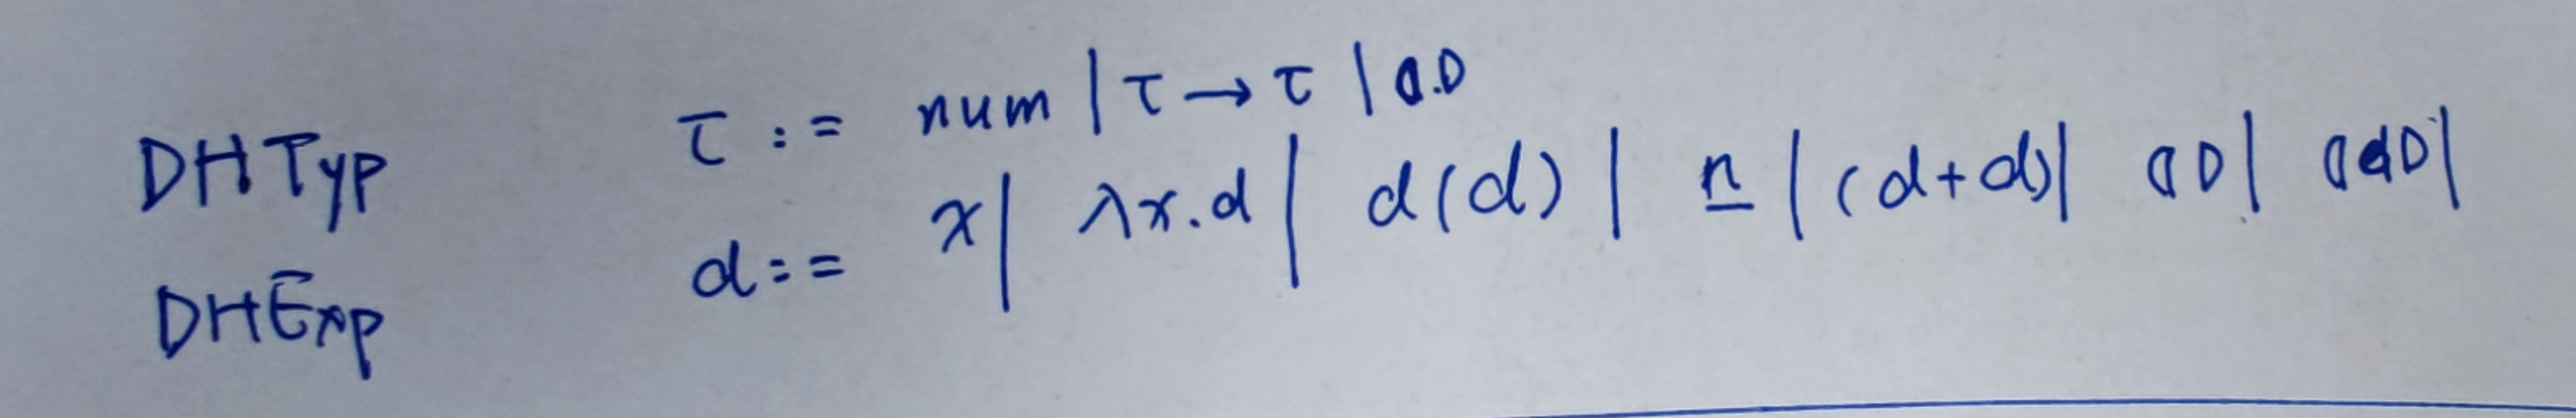
\includegraphics[width=0.7\textwidth]{syntax.png}
  \caption{Syntax}
  \label{fig:syntax}
\end{figure}

\begin{figure}[htbp]
  \centering
  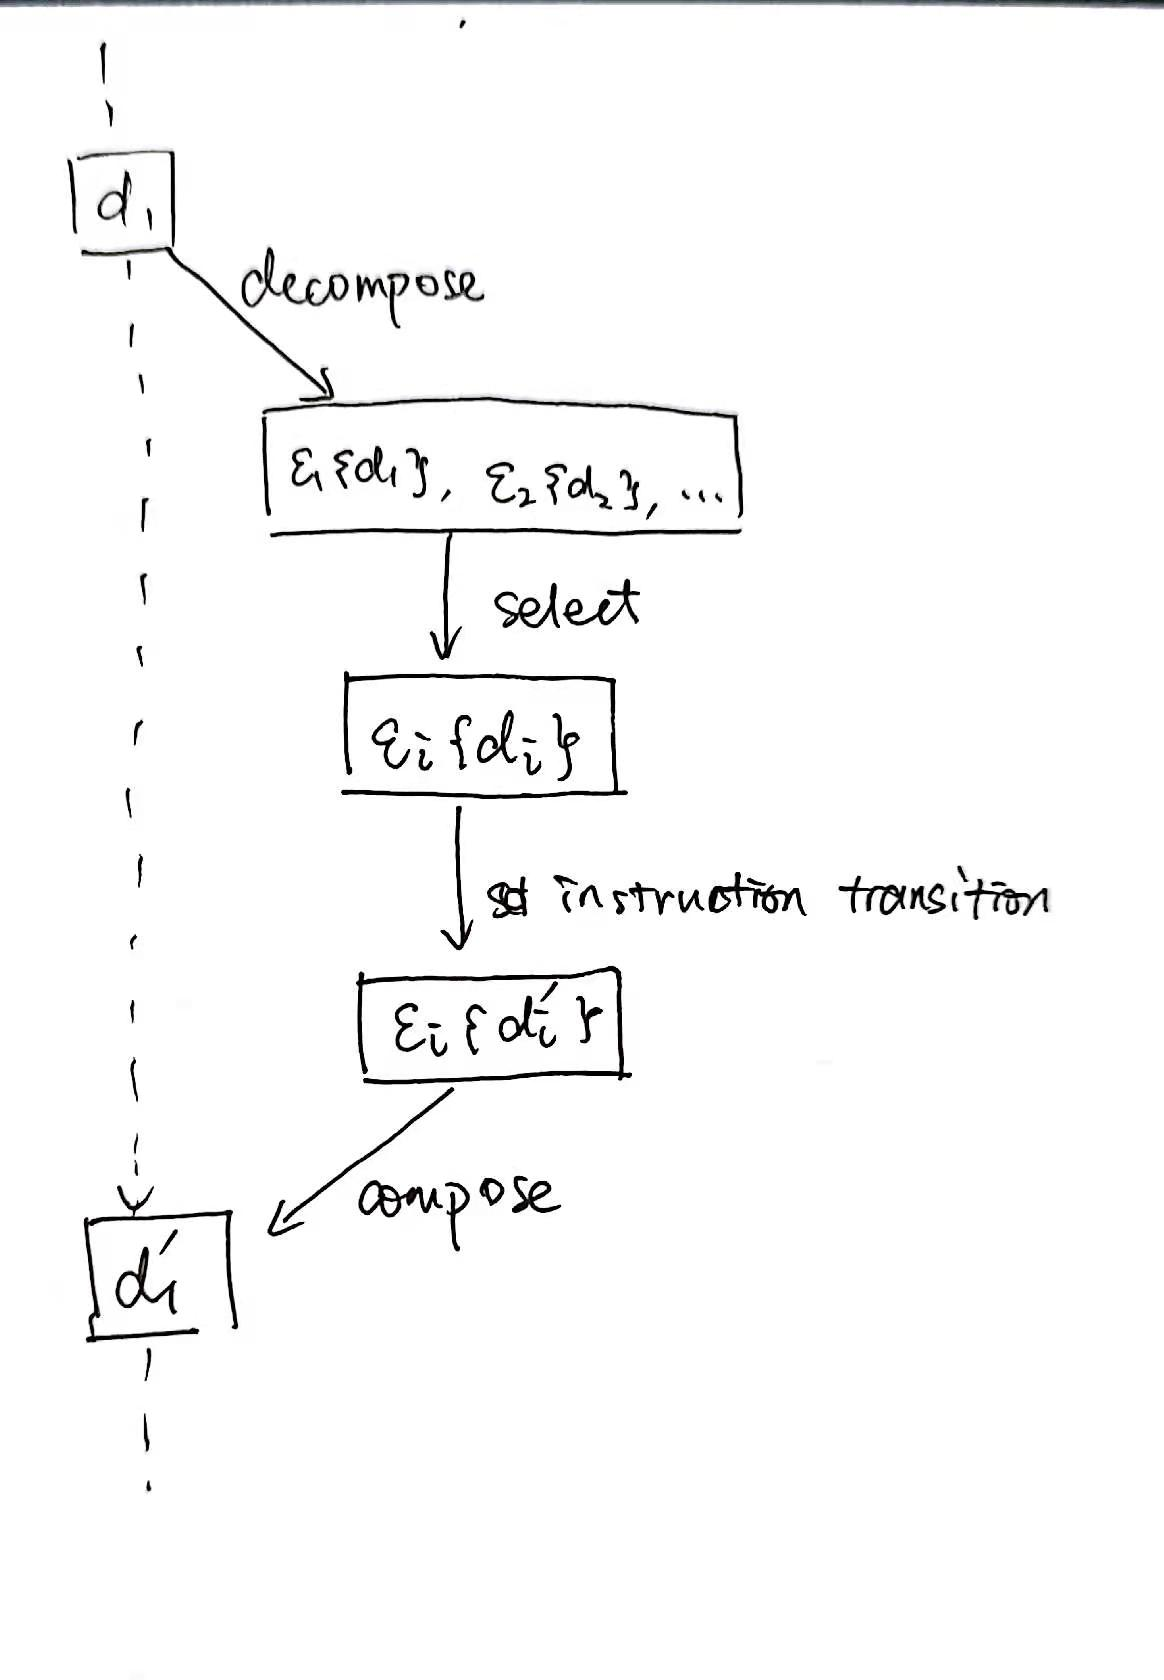
\includegraphics[width=0.5\textwidth]{structure.png}
  \caption{Sturcture of Stepper}
  \label{fig:structure}
\end{figure}

The structure of the stepper is shown in Figure \ref{fig:structure}. The expression is first decomposed into many independent evaluation contexts. Then, user may choose one of them to progress. And the stepper will compose them into the result then. For example, in Figure \ref{fig:multiple}, we have 3 evaluation contexts highlighted as green boxes. And when we click the second one, only the expression in second box is evaluated and composed into the whole expression.

Also, for some unnecessary steps, the stepper can detect it and then pause unless user click it manually. So, during the decompose, we need to detect this situation so that the stepper will not go on again. An example is shown in Figure []......

\begin{figure}[htbp]
  \centering
  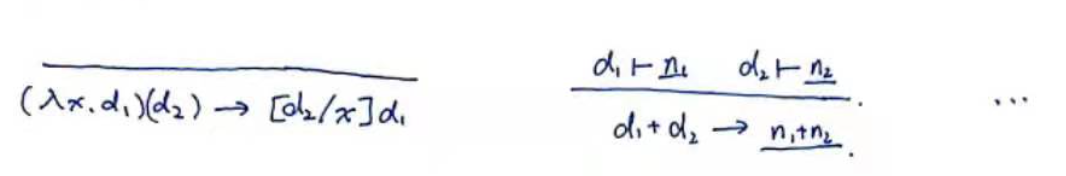
\includegraphics[width=0.7\textwidth]{instr_trans.png}
  \caption{Instruction Transition}
  \label{fig:instr_trans}
\end{figure}

We now formally define the instruction transition judgement. We use $d_1 \to d_2$ as instruction transition judgement. Figure \ref{fig:instr_trans} shows some of the transition judgement.

In Hazel, we have four types of expressions: boxed value, indeterminate, step, and paused. The instruction transition can be implemented to provide the type of the expressions. Therefore, we can easily know whether an expression is final, paused or steppable. %%TODO: not my works

Then, we have the evaluation context. Unlike the regular evaluation context, the decompose function will return a list of contexts. The recursive definition of the decompose function is shown in Figure \ref{fig:decompose}.

\begin{figure}[htbp]
  \centering
  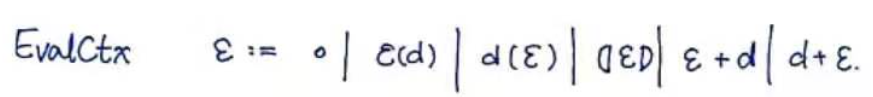
\includegraphics[width=0.7\textwidth]{context.png}
  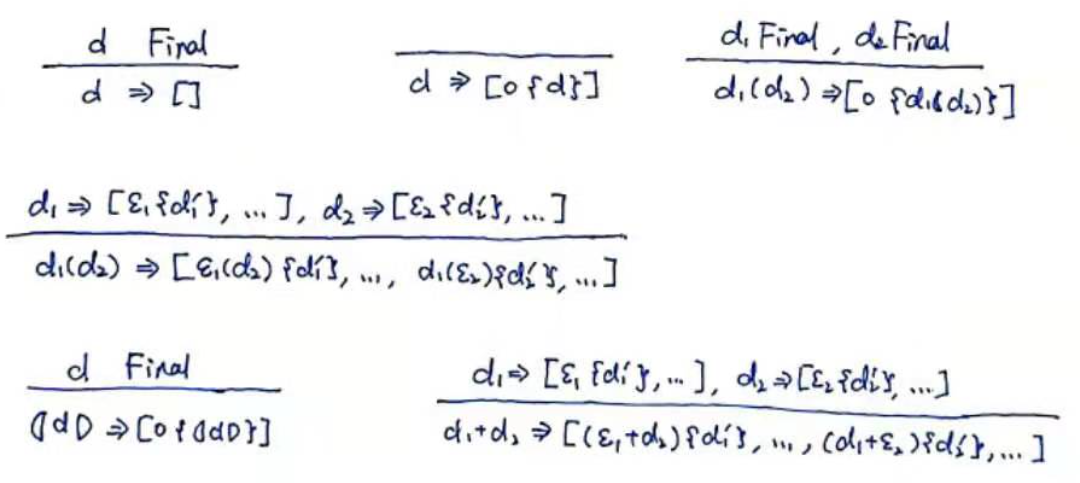
\includegraphics[width=0.7\textwidth]{decompose.png}
  \caption{Decompose}
  \label{fig:decompose}
\end{figure}

In conclusion, we first decompose the expression into many evaluation contexts for user to choose. Then, we run the instruction transition and compose the result to user. 